\section{Our implentation}
	The goal was to provide an interface to easily select data and plot results.
	We decided to create a website, which can easily be deployed on a web server or on a personal computer
	To do so, we decided to use Python as primary language, and Django for the web part.

	\subsection{Development process}
		After creating a basic interface to provide and display input data, we started the implementation of the algorithm.
		To test our results, we used basic automata (as shown in figure \ref{fig:automata}), with some probability transitions, to generate data streams.
		This way, we were able to compare streams from the same automata, or different ones, and therefore validating our results.

		\begin{figure}
			\begin{center}
				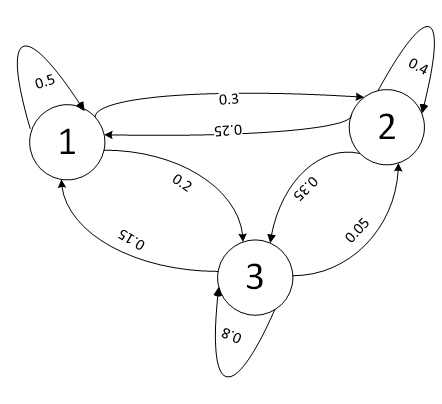
\includegraphics[width=0.8\textwidth]{figures/automata.png}
			\end{center}
			\caption{Example of an automata generating stream for us.}
			\label{fig:automata}
		\end{figure}

		Indeed, two streams from the same automata should have a deviation close to 0, when streams from differents automata should have a much higher deviation.

	